\ctable[caption={Studying a problem at multiple scales},
		label={fig:scales},
		width=5.5cm,
		figure]{c}{\tnote[]{Generic idea of renormalization. First the problem is solved at the
		largest scale. This block is divided into four sub blocks, where the process is repeated
		until unity is reached.}}{\FL
			\includegraphics[width=5cm]{fig/ising.png}
		\LL}
The heart of our method for solving the TSP problem is the renormalization
theory. The Renormalization Theory is originating from theoretical physics\cite{yoshiyuki1995nms}. In
theoretical physics Renormalization is used to study the observe the changes
in a physical system. The changes are observed by looking to the problem at
different scales. This idea is illustrated in figure \ref{fig:scales}. Here
the problem is divided into four parts initially. These parts on their own can
again be divided into four parts. This dividing process is repeated until the
scale is small enough to study the original problem.

This idea is mapped onto the Traveling Salesman problem. The total square in
figure \ref{fig:scales} can be seen as the total area where the cities are
located. When estimating the shortest route, it is first solved at the largest possible scale. 
This is followed by zooming into the problem until the estimated optimal tour is known. 
The procedure is illustrated in figure \ref{fig:renormalization}. Image 
\ref{fig:renormalization}A is the basic block. This basic block consists of four cells, 
which equals the partition of the problem into four parts. A cell
spans a part of the area and can be enabled or not. The cell is enabled (e.g.
needs to be visited) if one or more cities are located in the area spanned by
the cell.

The general idea of the algorithm is to solve the Traveling Salesman problem
for the larger block. This can be done easily, since a Traveling Salesman
problem for at most four cities can be easily solved without much performance
penalty, by simply enumerating all possibilities. When this is done, the TSP 
is solved at a smaller scale.

At the smaller scale, the estimated route is refined.
This can be seen in figure \ref{fig:iterations} and this is done by converting all the
cells into a basic block. In the basic blocks the shortest path can be found again.
However in this case there is an extra requirement. The path needs to start and finish
where the unrefined route crossed the border of the new basic block.

This refinement process is repeated until unity is reached. Unity is defined as the case 
where at most one city is located in each cell. In this case the estimated shortest route is
known. In the following subsections the algorithm is covered into more detail.

\subsection{Preprocessing step}
\ctable[caption={An illustration of how the Renormalization algorithm works},
	label={fig:renormalization},
	figure]{c}{\tnote[]{
	\begin{enumerate}
	\item[(A)] Determine the optimal route in a basic block. The dashed
	lines are the edges which can be traversed. The open circles are border
	points and the closed circles are cell points.
	\item[(B)] Based on the starting and end border node in a block, lookup the
	optimal path visiting the cells where at least one city is located.\\
	\item[(C)] Divide the block into four sub blocks(Each cell is converted into a basic block)
	, use the crossings of the route
	with the borders of a cell (The X) as new starting and end nodes.\\
	\item[(D)] These sub blocks are treated as a block again, and the process is repeated from
	picture B. This dividing continues until at most one city is located in each cell.
	\end{enumerate}}}{\FL
	\includegraphics[width=7cm]{fig/renormalization.pdf}
	\LL}

The preprocessing step reduces the amount of calculation needed each time the 
optimal route in a block is calculated. Basically this means that for
every possible configuration the optimal path is calculated, and stored in
a lookup table. There are two aspects which can be altered, the border point
at which the beginning and finish of the route is located and the visited
cells within the block.

For retrieving the shortest route through a block, it is considered as a
graph. The nodes are the border points and the cell points (Lying in the
centre of a cell). The nodes are connected by multiple edges. There are edges
between the border points and the closest cell points. There are also edges
from a cell point to the other edges. This set-up can be seen in figure
\ref{fig:renormalization}A. For retrieving the shortest route, a breadth first
search is used. Here all possible paths, without cycles, between the starting
and end node are calculated. Using these set of paths, the shortest routes
visiting subsets of cell points are searched.

\subsection{First iteration}
In the first iteration there is start with one basic block with four cells. In such a
block a subset of at least 3 cells needs to be occupied to create a starting
tour. The cells where at least one city is located, are connected to form a
shortest tour. This tour is an easy connection of the cities, and all the
possible routes between them do not need to be investigated.

\subsection{Further iterations}
When the first iteration is finished, the earlier blocks can be used to calculate an
approximation of the shortest tour at a smaller scale. The current cells can be 
converted into basic blocks by dividing them into four cells blocks in four sub
 blocks to study the problem at a smaller scale. Instead of
iterating over all the new basic blocks in the image, which can be quite time
consuming at a very small scale, only the blocks which contains at least
one city in the previous estimated shortest tour are used in the calculation.
This limits the amount of required memory in the order of the size of the problem.

The information which is retrieved from the previous scale are the crossing
points of the previous optimal path through the block. This optimal path can
be seen in figure \ref{fig:renormalization}B.  These crossing points are at
the places, where the edges of the path, pass the borders of one of the cells.
This is illustrated in figure \ref{fig:renormalization}C. These crossing
points, calculated in advance during the preprocessing stage, are used as start and
ending point in the sub block. The optimal path between the starting and
endpoint is retrieved, and placed in the sub block. The sub block is now a block
on its own again, and can be used in the next scale.

\subsection{Retrieving the estimate of the shortest tour}
This process, which looks like zooming in on a microscope, is repeated until
 unity is reached. Unity is defined as the case where each cell contains at most one
city. In this case the estimated shortest path can be retrieved directly by following 
the tour through the basic blocks.
In figure \ref{fig:iterations} the first four iterations of the algorithm on
$d198.tsp$ is shown. What is clear from this picture is that the route is
refined in each iteration, until it exactly maps on the estimation  of the
shortest optimal tour.

\ctable[caption={The first four iterations on d198.tsp},
		label={fig:iterations},
		width=7.5cm,
		figure]{cc}{\tnote[]{The renormalization starts with a basic form, a 
		square or a triangle. This slowly refines to the real tour through the 
		cities}}{\FL
			\includegraphics[width=3.5cm]{fig/it2.pdf} &
			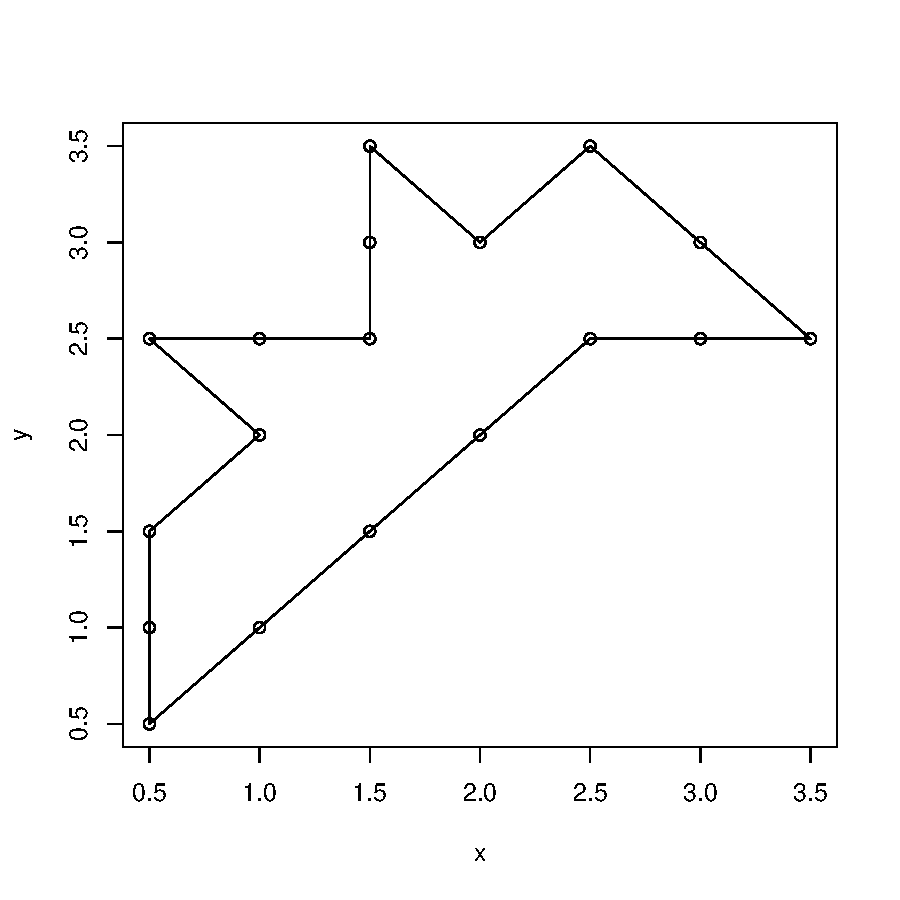
\includegraphics[width=3.5cm]{fig/it4.pdf} \NN
			\includegraphics[width=3.5cm]{fig/it8.pdf} &
			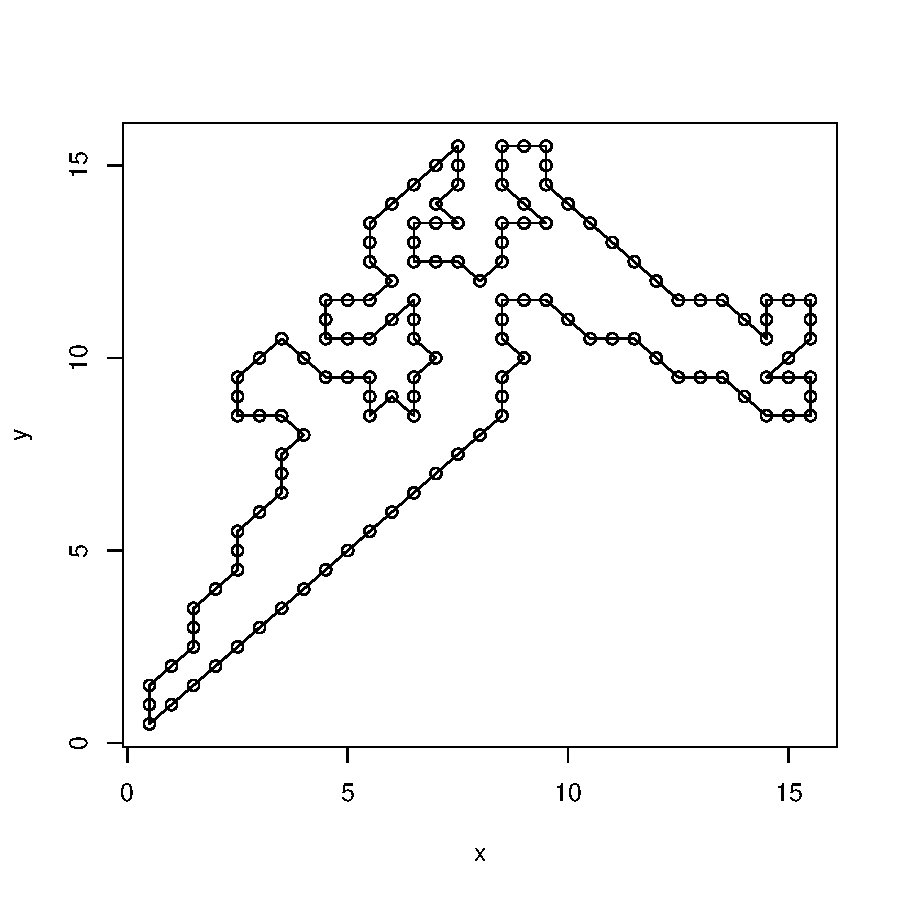
\includegraphics[width=3.5cm]{fig/it16.pdf} 
			\LL}

\subsection{Parallelization}
This algorithm can be extended for parallel execution. The foundation for
parallelism is in the observation that if the problem is decreased into a smaller scale, 
all the blocks are divided into four sub blocks independently. So if the code needs
to be parallelized the following approach can be taken:

\begin{enumerate}
\item First perform some iterations on a single process. This is done until
there are sufficient number of blocks for all the processes
\item Distribute the blocks over the processes, each process should have one
connected part of the tour.
\item Each process can now recursively divide these blocks into sub blocks,
until unity is reached.
\item The cities which are visited in the part of a single process are
retrieved and send back to the initiating process. The initiating process can collect the
data and output the total tour.
\end{enumerate}

This approach has a high potential of parallelism, since no communication is
needed. There is a pitfall however. If the blocks are shared equally it does
not have to mean that the work is equally divided. In a worst case scenario a
small group of processes can have a large set of all the cities. This problem
can be reduced if there is a process which performs load balancing by shifting
blocks, or sending one small set of blocks to a process at the time.

% vim:ft=tex:spell spelllang=en:autoindent
